%==============================================================================
%== template for LATEX poster =================================================
%==============================================================================
%
%--A0 beamer slide-------------------------------------------------------------
\documentclass[final]{beamer}
\usepackage[orientation=portrait,size=a0,
            scale=1.125        % font scale factor
           ]{beamerposter}

\geometry{
  hmargin=2.5cm, % little modification of margins
}

%
\usepackage[utf8]{inputenc}

\linespread{1.25}

%
%==The poster style============================================================
\usetheme{sharelatex}

%==Title, date and authors of the poster=======================================
\title
[Des enveloppes convexes, 2017-2018, Dijon, France] % Conference
{ % Poster title
Enveloppe convexe de points dans le plan Euclidien usuel
}

\author{ % Authors
Andrew LENC, Axel LE BOT
}
\institute
[Université de Bourgogne] % General University
{
ESIREM, France\\[0.3ex]
}
\date{\today}



\begin{document}
\begin{frame}[t]
%==============================================================================
\begin{multicols}{3}
%==============================================================================
%==The poster content==========================================================
%==============================================================================

\section{Introduction}

Dans un espace vectoriel E normé réel de dimension finie, on peut dire d'une partie C de E qu'elle est convexe si pour toutes paires de points pris dans C, le segment qui les connecte est entièrement contenu dans C.[1]

L'enveloppe convexe d'un ensemble de points fini est aussi l'ensemble de toutes les combinaisons convexes de ces points. C'est-à-dire qu'on peut réaliser une moyenne pondérée de ces points (tant que la somme des coefficients est égale à 1) et obtenir un point contenue dans l'enveloppe convexe, par conséquent l'enveloppe convexe sera l'ensemble de toutes ces moyennes. Ceci est décrit par la formule (1).
\begin{equation}
Conv(S) = \left \{  \sum_{i=1}^{|S|} \alpha_{i}x_{i} \left | (\forall i : \alpha_{i} \geqslant 0) \wedge  \sum_{i=1}^{|S|} \alpha_{i} = 1 \right \}
\end{equation}

Il est demandé dans le sujet de déterminer l'enveloppe convexe d'un nombre variable de points, dans le langage C ou C++, à l'aide de la bibliothèque OpenGL pour l'affichage.

\section{Algorithmes}

De nombreux algorithmes ont été écrits afin de résoudre le problème des enveloppes convexes, nous allons examiner le fonctionnement des plus connus, puis identifier et clarifier celui qui a été retenu afin de réaliser ce projet. On traitera, bien entendu, uniquement des algorithmes utilisés dans le cas planaire précisé par l'énoncé.
\subsection{Jarvis}
La marche de Jarvis[3] consiste à envelopper les points en trouvant un point appartenant à l'enveloppe, puis à continuer le long de celle-ci en cherchant le segment suivant ayant l'angle minimal avec le précédent. Il s'agit d'une des méthodes les plus intuitives, puisque comparable à envelopper les points dans, par exemple, du papier cadeau.

\subsection{Graham}
Le parcours de Graham[2] trouve d'abord le point de plus petite ordonnée (départagé par l'abscisse la plus basse), puis il trie les points en fonction de l'angle du segment qui les relie à P et l'axe des abscisses. Ensuite, pour chaque triplet de points successifs dans le tableau précédemment créé, l'algorithme détermine s'il s'agit d'un "tournant à gauche" ou "à droite", et exclut le point du milieu dans le cas d'un tournant à gauche (puisque les points sont parcouru dans le sens horaire).

\subsection{QuickHull}
L'algorithme détermine d'abord les points avec les abscisses la plus basse et la plus haute, puisque ceux-ci font toujours partie de l'enveloppe convexe, puis il divise l'ensemble des points en deux ensemble de chaque côté de l'axe, ceux-ci seront traités de façon récursive.[4] Pour chaque partie, l'algorithme détermine le point le plus éloigné de l'axe, grâce à celui-ci, on peut déterminer un triangle avec les deux autres points déterminés plus tôt et conclure que les points à l'intérieur du triangle ne font pas partie de l'enveloppe. On répète ensuite cette étape sur les deux nouveaux axes obtenus par les ligne du triangle. L'algorithme finit lorsque le tableau de points à traiter est vide.

\subsection{Chan}

Il s'agit d'un des algorithmes les plus complexes dans l'exécution, mais un des plus optimisés. Il consiste à diviser l'ensemble de points en plus petits ensemble et à en calculer l'enveloppe convexe grâce au parcours de Graham, puis à calculer l'enveloppe convexe des enveloppes calculées grâce à la marche de Jarvis.[5]

\subsection{Andrew}
Cet algorithme trie d'abord les points par leur abscisees, et les départage par leur ordonnée, puis construit deux "coques", une supérieure, qui démarre au point le plus à gauche et finit au point le plus à droite, et une inférieure qui constitue le reste de l'enveloppe. Dans chaque coque, l'algorithme détermine les points à choisir en parcourant la liste triée, et en comparant les angles des segments, de manière similaire à la marche de Jarvis. [6]

\vskip1ex
\begin{figure}
\centering
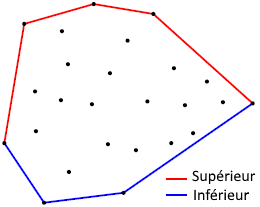
\includegraphics[width=0.99\columnwidth]{UpperAndLowerConvexHulls.png}
\caption{Principe des deux "coques" de l'algorithme de Andrew }
\end{figure}
\vskip2ex

\subsection{Comparatif}
On compare la complexité des algorithmes les plus connus. n étant le nombre de points que doit traité l'algorithme, alors que h est le nombre de points finalement contenus dans l'enveloppe convexe. La première ligne décrit la complexité théorique, tandis que la seconde précise la pire complexité à laquelle on peut s'attendre, en fonction de la nature des points à traiter (symétrie, groupement, etc).
\vskip1ex
\begin{table}
\centering
\caption{Comparatif des complexité des différents algorithmes}
\begin{tabular}{ccccc}
\hline\hline
Jarvis & Graham & Chan & QuickHull & Andrew\\
\hline
o(hn) & O(n log n) & O(n log h) & O(n log n) & O(n log n)\\
o(n²) & O(n log n) & O(n log n) & O(n log n) & O(n log n)\\
\hline\hline
\end{tabular}
\end{table}
\vskip2ex

\section{Autour du programme}

\subsection{Glut}

La librairie (API) d'openGL nous permet d'implémenter les fonctions gérant le cycle de vie de l'application ainsi que ses fonctionnalités principales (clic, etc, ...).

Configuration des fonctions de glut :
\begin{itemize}
 \item glutMainLoop : Fonction de lancement glut
 \item glutIdleFunc : Fonction utilisée quand le programme n'effectue pas de tâches
 \item glutDisplayFunc : Fonction d'affichage
 \item glutReshapeFunc : Fonction de redessinnage
 \item glutKeyboardFunc : Fonction utilisé pour les évènements d'entrées clavier
 \item glutSpecialFunc : Fonction utilisé pour les évènements d'entrées spécial du programme
 \item glutMouseFunc : Fonction utilisé pour les évènements d'entrées de la souris
 \item glutMotionFunc : Fonction utilisé pour les évènements de mouvement de la souris
\end{itemize}

Configuration des comportements de glut :
\begin{itemize}
 \item glOrtho : Décrit une transformation que produit une projection parallèle
 \item glViewPort : Décrit la zone d'affichage du rendu
\end{itemize}

\subsection{Logique}
Nous avons du, après avoir lu la documentation de la librairie, implémenter les différentes fonctions nécessaire à glut (vu précédemment), ainsi le cycle de vie et la configuration de l'application était géré.
Petit à petit les fonctions ont été codés pour dessiner des points ou dessiner des segments. Le dessin s'organise en calque, les index permettent à OpenGL de savoir dans quel ordre dessiner les différents éléments.

Derrière nous avons rajouter la logique souhaité du projet permettant dans openGL d'ajouter des points à l'aide de la souris, de stocker ses points et de les traiter à l'aide de l'algorithme choisie pour en faire une enveloppe convexe.

Deux listes de points seront utilisées, une pour l'affichage et une autre pour le stockage.

Au cours du développement il a été utile d'ajouter un logger permettant de mettre en place des logs de différents niveau afin de debuguer ou mettre en garde l'utilisation de l'application. Vous trouverez ces traces en commentaires dans le code.

\subsection{Commandes}
\begin{itemize}
    \item  Clic gauche ajout d'un point a l'emplacement du curseur
    \item Clic droit :
    \begin{itemize}
        \item  Menu contextuel (activation/désactivation de l'affichage des points à l'intérieur de l'enveloppe convexe
        \item Choix de l'algorithme de l'enveloppe convexe
        \item Ajout manuel de point via la console
    \end{itemize}
    \item Clic du milieu : suppression du point à l'emplacement du curseur
    \item CTRL + (+/-) ou CTRL + Molette: zoomer/dézoomer
    \item D : suppression du dernier points ajouté
    \item R : réinitialisation de l'application
    \item Q : Fermeture de l'application
    \item Flèches : Déplacement de l'affichage
\end{itemize}

\subsection{Squelette}
\begin{itemize}
    \item main.cpp : Contient la logique principale du programme et l'implémentation d'openGL.
    \item tools.cpp : Contient des fonctions utilitaires permettant de simplifier le code principale.
    \item algorithm.cpp : Contient les algorithmes permettant de calculer l'enveloppe convexe de points passés en paramètres.
Il contient pour le moment uniquement l'algorithme de Chaine monotone mais il est facile d'y ajouter d'autre et de les rendre accessibles dans l'interface.
\end{itemize}

%==============================================================================
%==End of content==============================================================
%==============================================================================

%--References------------------------------------------------------------------

\subsection{Bibliographie}

\begin{thebibliography}{99}
\bibitem{ref1} Université d'Angers, \textit{http://enseignement.math.univ-angers.fr/documents/MEF1_geom1/convexite.pdf}

\bibitem{ref2} Page sur le parcours de Graham de Wikipedia, \textit{https://fr.wikipedia.org/wiki/Parcours_de_Graham}

\bibitem{ref3} Page sur la marche de Jarvis de Wikipedia, \textit{https://fr.wikipedia.org/wiki/Marche_de_Jarvis}

\bibitem{ref4} Page sur l'algorithme QuickHull de Wikipedia en anglais, \textit{https://en.wikipedia.org/wiki/Quickhulln}

\bibitem{ref5} Page sur l'algorithme de Chan de Wikipedia, \textit{https://fr.wikipedia.org/wiki/Algorithme_de_Chan}

\bibitem{ref6} Page sur l'algorithme Monotone Chain de Wikibook, \textit{https://fr.wikipedia.org/wiki/Algorithme_de_Chan}


\end{thebibliography}
%--End of references-----------------------------------------------------------

\end{multicols}

%==============================================================================
\end{frame}
\end{document}
